\documentclass[11pt]{article}
\usepackage[margin=0.85in]{geometry}
\usepackage{amsmath,amssymb,graphicx}
\pagestyle{empty}

\begin{document}
\begin{center}
  {\Large\bfseries Estimating a nonlinear ODE coefficient in \(L^2\)}\\[3pt]
  22 November 2026
\end{center}

\noindent\textbf{Model.} On \(0\le t\le 1\), the trajectory and target coefficient satisfy
\[
  \dot x^\ast(t)=\theta^\ast B^\ast(t), \qquad
  B^\ast(t)=x^\ast(t)^2+t, \qquad x^\ast(0)=0.4, \quad \theta^\ast=0.8.
\]
At \(t_i=(i-1)/(n-1)\), both methods use the same observations
\(Y_i=x^\ast(t_i)+\sigma\varepsilon_i\), with independent \(\varepsilon_i\sim N(0,1)\).
A dense DOP853 solution supplies \(x^\ast\) for data generation and error evaluation.

\medskip
\noindent\textbf{Estimators.} Method A fits a local line at each \(t\) by Gaussian kernel weighting,
\[
  (\widehat a_t,\widehat b_t)=\arg\min_{a,b}\sum_{i=1}^n
  \exp\!\left[-\frac{(t_i-t)^2}{2h_n^2}\right]
  \bigl(Y_i-a-b(t_i-t)\bigr)^2, \qquad h_n=0.48\,n^{-1/5}.
\]
It uses the fitted intercept to form \(\widehat B_n^A(t)=\widehat a_t^2+t\).
For this smooth trajectory, the intercept's bias \(O(h_n^2)\) and standard deviation
\(O((nh_n)^{-1/2})\) are both of order \(n^{-2/5}\).
Method B linearly interpolates the raw values \(\widehat B_n^B(t_i)=Y_i^2+t_i\).

\medskip
\noindent\textbf{Evaluation.} For each replication we computed
\(E_n^M=(\int_0^1|\widehat B_n^M(t)-B^\ast(t)|^2\,dt)^{1/2}\)
using Simpson quadrature at the endpoints and midpoint of every observation interval.
We averaged 300 such errors per setting (seed 2026). For each method and noise level,
the exponent \(p\) is the negative slope of \(\log\bar E_{n,\sigma}^M\) against \(\log n\)
over \(n=50,100,200,400,800,1600\).

\begin{figure}[!ht]
  \centering
  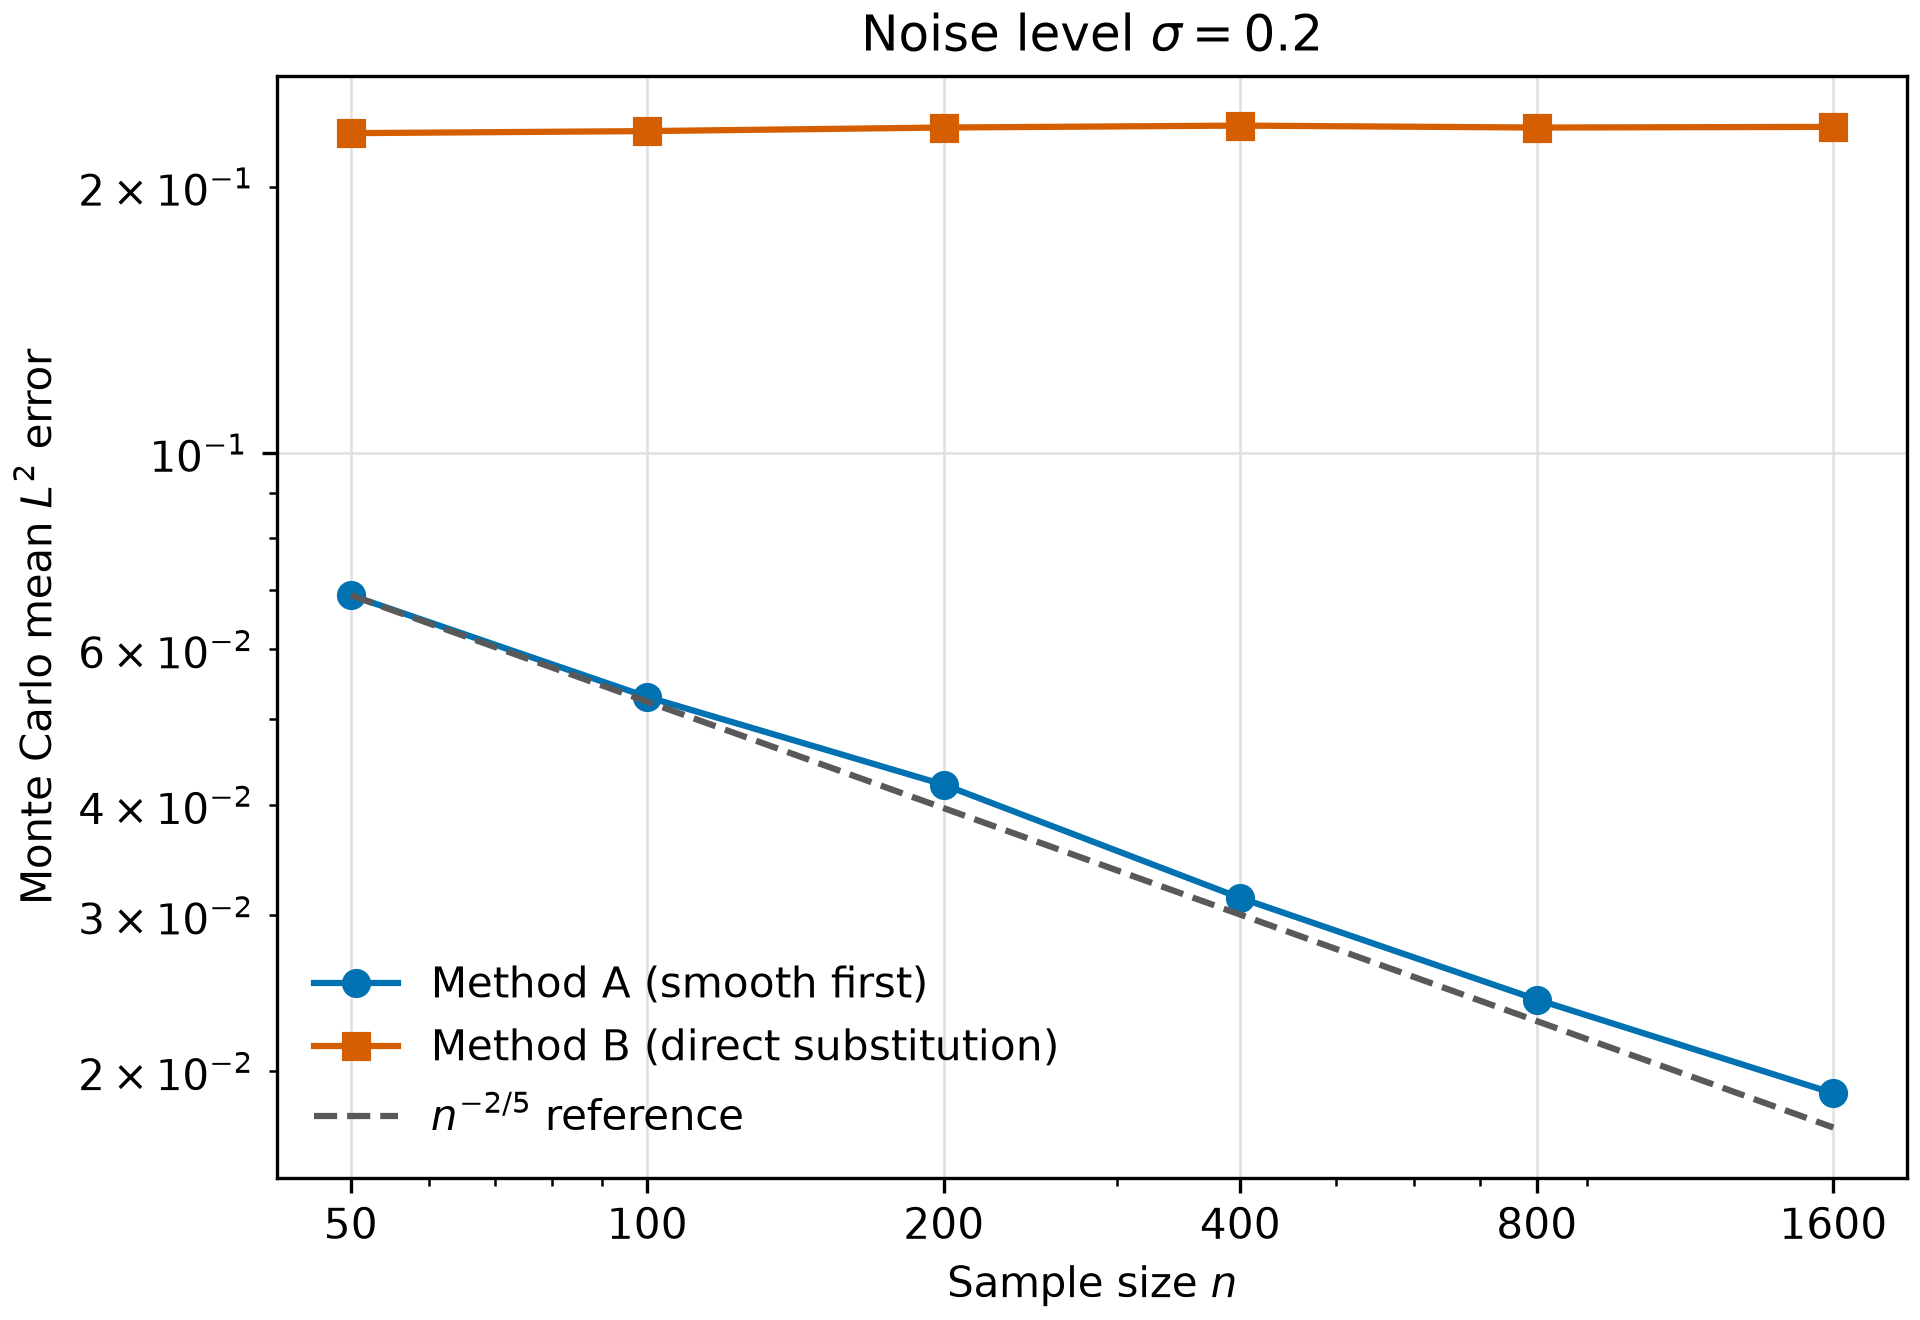
\includegraphics[width=.49\linewidth]{results/L2_error_sigma_0.2.png}\hfill
  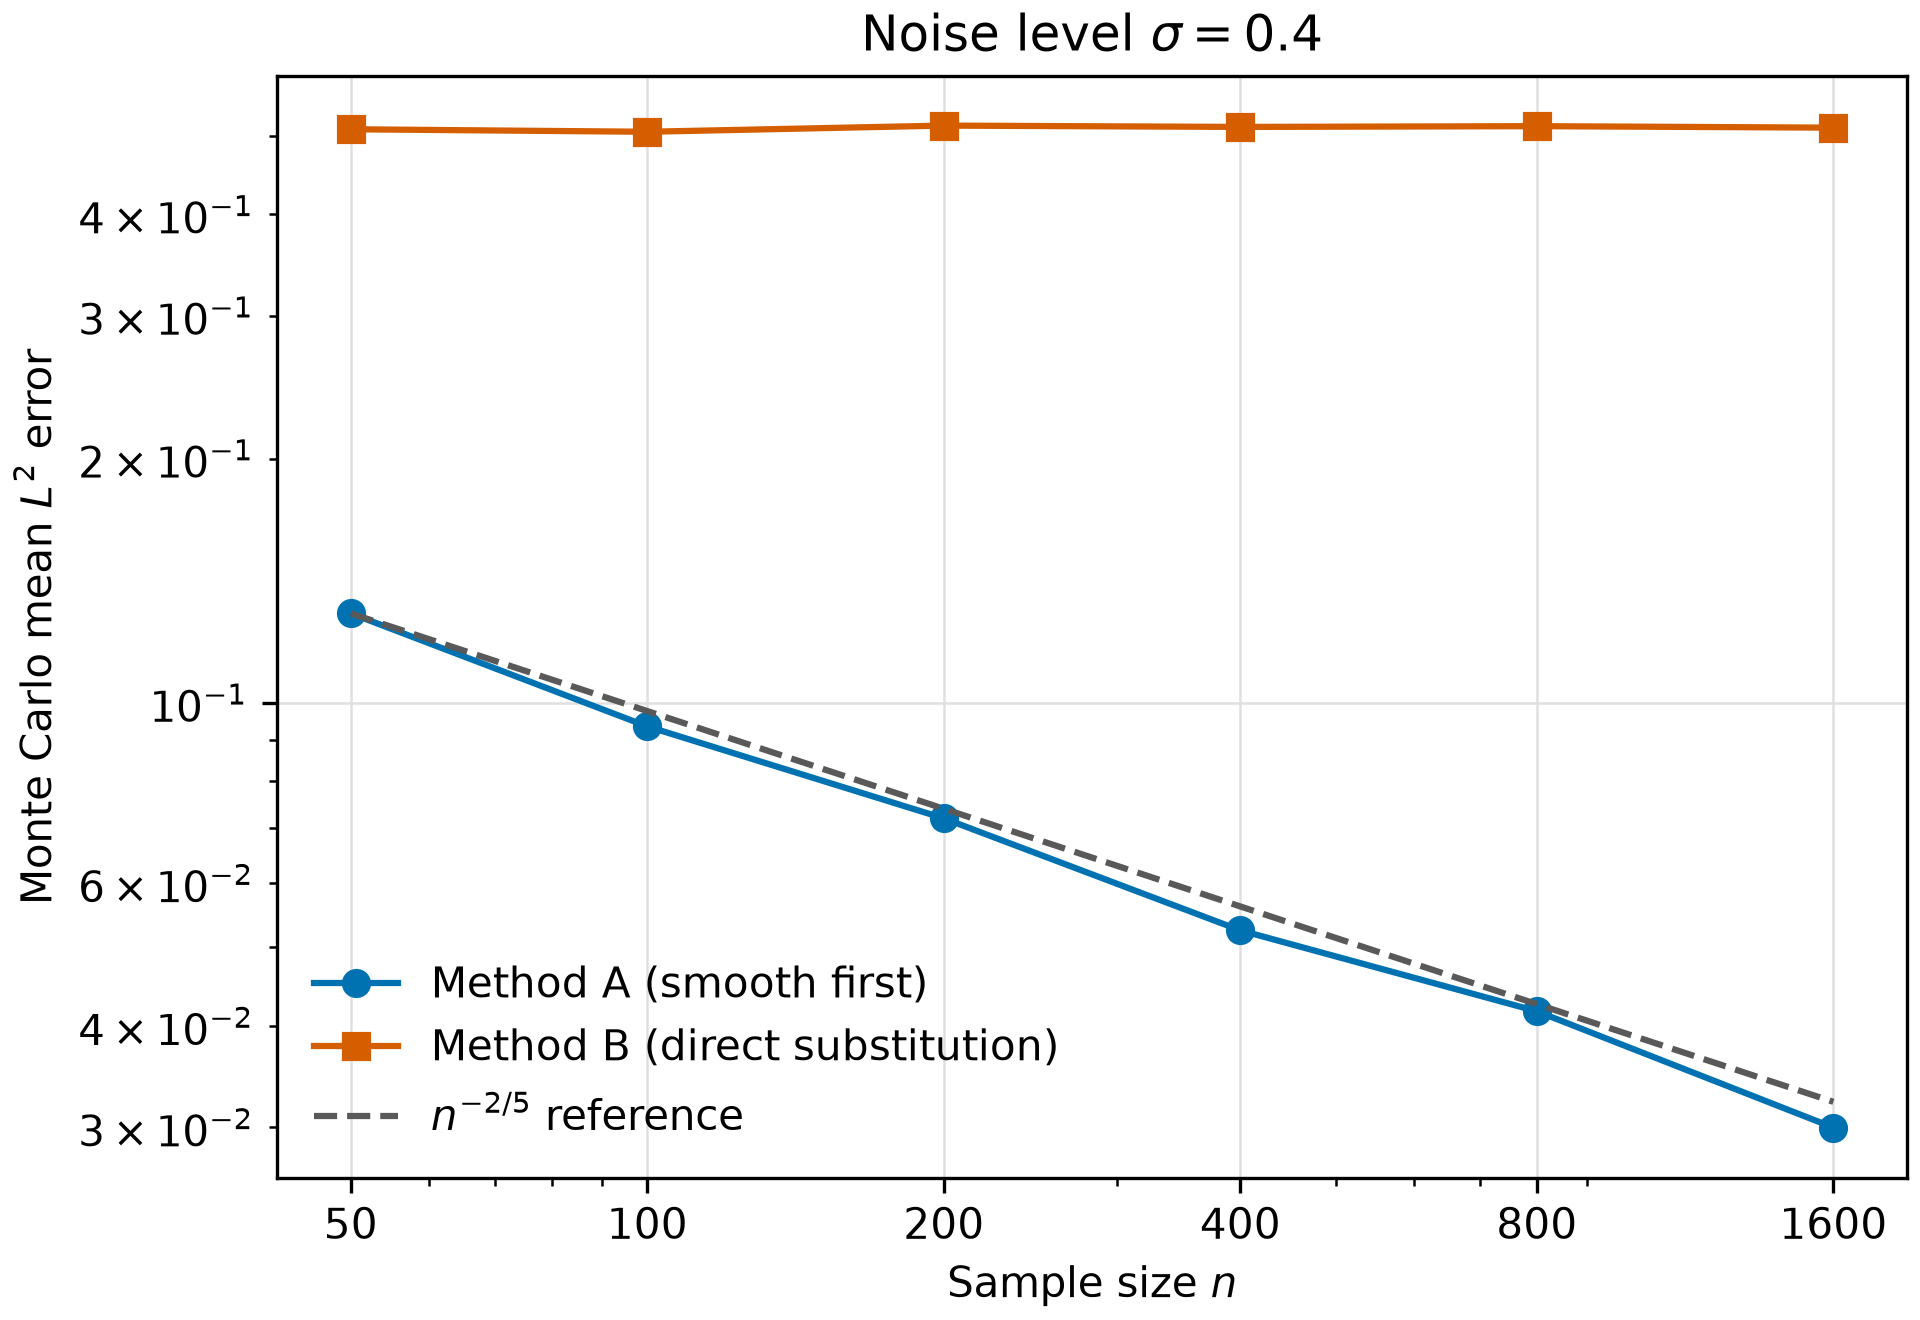
\includegraphics[width=.49\linewidth]{results/L2_error_sigma_0.4.png}
  \caption{The dark gray dashed line is
  \(r_\sigma(n)=\bar E_{50,\sigma}^A(n/50)^{-2/5}\).
  It starts at Method A's measured mean error at \(n=50\). Its fixed log--log slope
  of \(-0.4\) shows the benchmark decline of about \(24\%\) each time \(n\) doubles.}
\end{figure}

\noindent\textbf{Findings.} At \(\sigma=0.2\) and \(0.4\), respectively, Method A's
exponents were \(0.377\) and \(0.414\), consistent with \(L^2\) convergence to
\(B^\ast\) at rate \(n^{-2/5}\). Method B's mean errors stayed near \(0.23\) and
\(0.51\), with exponents \(-0.0047\) and \(-0.0027\).
Indeed, \(\mathbb E[Y_i^2+t_i]=B^\ast(t_i)+\sigma^2\).
The interpolant integrates to a trapezoidal average of independent node values, so
\(\int_0^1(\widehat B_n^B-B^\ast)\,dt\xrightarrow{p}\sigma^2\).
The \(L^2\) error bounds the absolute value of this integral from above,
ruling out convergence to \(B^\ast\) for fixed \(\sigma>0\).
\end{document}
